\documentclass[11pt]{article}

% ============================================================================
%  Rub' al-Khali soil metagenome -- MANUSCRIPT v2, rewritten 2026-09-17.
%  v1 is archived at main_v1.tex and no prose is carried over from it.
%  Every number traces to notes/CATALOGUE_NUMBERS.md; corrections and their
%  reasons are in notes/CORRECTIONS.md; how each analysis works is in
%  notes/dossiers/. Numbers not yet registered are marked with the unreg macro.
% ============================================================================

\usepackage[a4paper,margin=2.4cm]{geometry}
\usepackage{graphicx}
\usepackage{booktabs}
\usepackage{array}
\usepackage{xcolor}
\usepackage[numbers,sort&compress]{natbib}
\usepackage{hyperref}
\hypersetup{colorlinks=true,linkcolor=blue!50!black,citecolor=teal!60!black,urlcolor=blue!50!black}
\setlength{\emergencystretch}{2em}

\providecommand{\todo}[1]{\textcolor{red}{\textbf{[TODO: #1]}}}
\newcommand{\unreg}[1]{\textcolor{orange!80!black}{#1}}   % computed, not yet registered

\title{\textbf{Known phyla, unknown proteome:\\ a controlled census of the Rub' al-Khali soil metagenome}}
\author{A. Lopez Velazquez \textit{et al.}\\ \small King Abdullah University of Science and Technology}
\date{}

\begin{document}
\maketitle

% ============================================================================
\section*{Abstract}
% 150 words, unreferenced. Written last; this is the working version.
Most microbial proteins match no characterised family, and a pooled catalogue cannot say whether
that unknown fraction is biology or artefact, nor why it is unknown. We shotgun sequenced 551 soil
samples from 60 sites across the Rub' al-Khali on five expeditions over 31 months and recovered
5{,}438 species-level genomes, all in named phyla. A tenth of their protein clusters (9.89\%) have
no reference homolog. These form 106{,}042 families, 79.4\% recurring in all five expeditions,
under purifying selection. In 23 species also cultured from these soils, cultured and metagenome
genomes share 80\% of their annotated proteins but 16\% of their dark ones: dark proteins are
strain-variable content that a few reference genomes never capture.
Lineage, not assembly quality, sets how dark a genome is; 237 species in two Thermoplasmatota
classes are four to six times darker than matched genomes and carry a fifth of the dark families.
The unknown proteome is the accessory genome of lineages without reference strains, which is why
biome-matched references recover more of it than databases five times larger.

% ============================================================================
\section*{Introduction}

Drylands cover roughly two fifths of the land surface and are projected to expand
\citep{huang2016dryland,maestre2015aridity}, and their hot hyperarid interiors are the low-biomass
case in which contamination approaches the detection limit \citep{contamination2025guidelines}. The
Rub' al-Khali, the largest contiguous sand sea, had no genome-resolved microbial survey. A companion
16S rRNA survey of the same transect mapped its bacterial ecology by landscape, soil position and
rainfall\todo{cite the companion ecology manuscript (Tawfiq et al.); no bibkey yet}, and listed what
amplicons cannot reach: gene content without primer bias, function tied to a genome, and the archaea.

What genomes reveal is mostly unknown. Across global catalogues a large share of microbial protein
families match no characterised family, and the size of that share depends on the reference and
the rule used to call it \citep{pavlopoulos2023darkmatter,vanni2022agnostos,coelho2022gmgc}. The
unknown families are numerous, span species, evolve under purifying selection and concentrate in
uncultivated lineages \citep{rodriguezdelrio2024fesnov}; most are restricted to one ecosystem
\citep{aplakidou2025quadrupling}; and at the structural level fold space is near saturation, so
residual novelty lies in how known domains are combined \citep{lau2024ted,yeo2025afesm}. These
catalogues report reference absence with a lineage attached. They do not report whether a family
persists in one place over time, which environment sorts it, whether closed genomes of the same
species carry it, or how often the calling procedure errs on proteins that are already known.

Two design limits of pooled catalogues produce those gaps. Pooling strips context: a family drawn
from thousands of studies has no repeated sampling, no measured chemistry and no cultured neighbour
against which to test whether it is biology or artefact. And the error rate is unmeasured: a no-hit
against a reference is reported as novelty without a matched set of known proteins passed through
the same procedure to show how often it returns no-hit when it should not.

Here we address both limits in one biome. We shotgun sequenced 551 soil samples from 60 sites across
the Rub' al-Khali on five expeditions over 31 months, at three soil positions and with elemental
chemistry, recovered 5{,}438 species-level genomes, and measured the unknown fraction of their
proteome against a control at every layer: matched annotated families for recurrence, selection and
reference absence; long-read genomes of strains cultured from soils of the same basin; blinded
known-fold controls for structure; and a matched null for the lineage that carries most of it. The
organisms are ordinary at every rank above order. Their proteome is not, and the gap lies in the
reference set rather than in the organisms.

% ============================================================================
\section*{Results}

\subsection*{The organisms are ordinary at every rank above order}

We sampled 60 sites along a 1{,}043~km transect of the Rub' al-Khali on five expeditions between
March 2023 and October 2025, at the soil surface, in the subsurface and beside plant roots, and
shotgun sequenced 551 soil samples to a median depth of 21.58~Gbp per sample (Fig.~\ref{fig:design}a--c).
Of the 549 samples that assembled, two SemiBin2 binnings (pretrained model and self-supervised)
refined by DAS\_Tool yielded 14{,}426 bins, 4{,}225 of them high quality and 8{,}209 medium quality
by completeness and contamination alone; dereplication at 95\% average nucleotide identity gave
5{,}438 species representatives, 2{,}259 high quality and 3{,}179 medium quality
(Fig.~\ref{fig:design}d). Taxonomy throughout is GTDB release 232.

Every representative was placed to class rank, within 51 named phyla. The first rank without a
named taxon was order for 11 representatives, family for 142, genus for 1{,}343 and species for
3{,}755; 187 carry a named species (Fig.~\ref{fig:design}e). These are mutually exclusive depths of
the first empty rank, not counts of validated new taxa. Of the 11 order-level gaps, the 10 with
adequate marker coverage were chimera-clean by GUNC (clade separation 0.01 to 0.32 against a 0.45
threshold), and de novo trees with release-calibrated relative evolutionary divergence supported no
new order: six are single-genome lineages and the two multi-genome clades sit at genus and family
depth.

\subsection*{A tenth of the genome-resolved protein clusters have no reference homolog, and they behave as coding sequence}

Gene prediction on the 552 assembly files gave 753{,}305{,}533 proteins, which collapsed to
449{,}265{,}306 cluster representatives at 90\% identity over 80\% of the length. A cluster was
called sequence-dark when none of its searched members returned a UniRef50 hit under a sensitive
search with an E-value threshold and no identity or coverage filter (Methods); 69{,}938{,}628
representatives (15.6\%) were dark. Restricting to clusters with at least one member on a contig of
the 37{,}949 medium- or high-quality bins of the two binnings before refinement gives the
genome-resolved census: 4{,}292{,}446 of 43{,}423{,}322 representatives (9.89\%) have no reference
homolog (Fig.~\ref{fig:dark}a). Both percentages are shares of cluster representatives, not of
proteins or of species. Length, not assembly completeness, separates dark from annotated clusters:
76\% of dark representatives are shorter than 100 residues against 30\% of all representatives,
while partial gene calls are equally common in both (86.7\% and 87.5\%) (Fig.~\ref{fig:dark}b).

Four tests separate encoded biology from spurious open reading frames; the first defines the family
set and the other three test it. Recurrence: clustering the 4{,}292{,}446 dark representatives at
50\% identity and admitting only families with at least three diverged members from at least three
samples and two sites gave 106{,}042 dark families holding 536{,}437 genes; the 782{,}616 clusters
with one or two variants and the 2{,}784 within-genome paralog sets were excluded. The median
admitted family was assembled in 12 samples at 9 sites.

Persistence: with reads from all 551 samples mapped to the member genes, the median family is
detected in 98 samples, four families are confined to one sample, and 79.4\% of families are detected
in all five expeditions (94.8\% in at least four). Under the stricter criterion of independent
assembly, 28.9\% were assembled in all five (Fig.~\ref{fig:dark}c). Detection by covered fraction
favours short genes, and persistence holds within every length stratum: 67.1\% of families with
representatives of at least 250 residues are detected in all five expeditions.

Selection: the median pairwise dN/dS across 97{,}200 evaluable dark families is 0.425, with 96.7\%
below one, against 0.388 (99.6\% below one, $n = 95{,}647$) for 106{,}042 UniRef50-matched families
matched on representative length and family size and passed through the identical clustering,
alignment and estimation steps (Fig.~\ref{fig:dark}d). The dark families are measurably less
constrained than the matched control. The null is the same sequences read in the wrong frame: on a
seeded subset of 10{,}000 dark families, the member genes shifted by one nucleotide (stop codons
masked) give a median pairwise dN/dS of 1.087 (37.7\% below one), while the identical families in
their annotated frame give 0.427 (97.0\% below one), and the shifted frame is the higher of the two
in 92.4\% of families. The annotated frame of the dark families is therefore the selected one, under
purifying selection of the same kind and order as known genes measured on the same instrument. A set
dominated by spurious calls would not behave this way.

Cultivation is the fourth test. Long-read genomes of 722 strains cultured from saline pans, oases
and campground soils of the same basin were called dark by the identical UniRef50 rule. They share a
species (average nucleotide identity $\geq 95\%$) with 25 of the 5{,}438 representatives, giving 23
species pairs. The cultured genomes were slightly less dark, lower in 18 of 23 pairs by a median
$0.33$ percentage points (Wilcoxon $p = 0.021$), and 40.9\% of the dark proteins of these cultured
genomes reappear as dark representatives in the catalogue (Fig.~\ref{fig:dark}e). Dark proteins in
these near-complete genomes (median two contigs) are shorter than in the catalogue (median 59 against
70 residues), so fragmented assembly does not explain their length. Matched protein by protein, the
two genomes of a pair are one proteome for their annotated content and two for their dark content:
80\% of annotated MAG proteins have a reciprocal partner in the culture at a median 99.7\% identity,
against 16\% of dark proteins, in 23 of 23 pairs in both directions and unchanged on complete calls
of at least 100 residues. The MAG-unique remainder is short, partial and contig-terminal; the
culture-unique remainder is longer, rarely dark and enriched in phage, transposase and conjugation
proteins. The dark proteins of a species are therefore its strain-variable accessory content, which
is why a few reference strains per species do not capture them. This control reaches only cultivable, well-referenced
bacteria whose dark rate is about 1\% of proteins; it does not reach the archaea.

\subsection*{Lineage, not genome quality, sets how much of a genome is unknown}

Per genome, the dark fraction is the share of protein instances on a representative's contigs whose
cluster has no UniRef50 homolog; across the 5{,}438 representatives its median is 6.3\%
(interquartile range 3.7--10.4\%), a per-genome rate. Assembly quality (completeness, contamination, N50 and length together) explains 11.5\% of the
variance in that fraction. Adding phylum raises the explained share to 76.8\% and genus to 83.5\%;
72.0\% of the variance is unique to lineage and 2.0\% unique to quality (Fig.~\ref{fig:lineage}a).
Larger genomes are slightly less dark ($-0.096$ per tenfold increase in corrected size, $R^2$ 0.067),
so genome size does not explain darkness. Taxonomic novelty predicts part of it: the median dark
fraction falls from 0.217 for genomes unnamed at phylum to 0.017 for genomes named to species
(Fig.~\ref{fig:lineage}b), and within Actinomycetota, Pseudomonadota and Bacteroidota genomes with a
placeholder genus are darker than those with a named genus (medians 0.075 against 0.022, 0.051
against 0.030, 0.068 against 0.053). That much is expected, because a lineage absent from UniRef50
is dark by construction. Novelty does not absorb the lineage term: with first unnamed rank in the
model, phylum still adds 0.340 to $R^2$, 52\% of its unconditioned increment. Phylum and genus enter
with far more degrees of freedom than the four quality covariates and the model treats genomes as
independent draws, so these increments are descriptive upper bounds; the like-for-like test is the
matched contrast in the next section.

The residual is concentrated. After the quality model, Thermoplasmatota genomes are 0.21 darker than
predicted, Cyanobacteriota 0.14 and Bdellovibrionota 0.10, while Halobacteriota, Bacillota,
Pseudomonadota and Actinomycetota sit below the line (Fig.~\ref{fig:lineage}c). The largest single
owner of the unknown proteome is one archaeal phylum.

\subsection*{Two poorly sampled archaeal classes carry a fifth of the attributable dark families}

The catalogue holds 237 Thermoplasmatota species: 185 in class SW-10-69-26, 51 in class E2 and one
in Thermoplasmata, none with a named genus. GTDB release 232 holds 21 and 197 species
representatives in the two classes, fewer together than this one sand sea. Their median dark
fraction is 0.310, against 0.046 for the other 354 archaea and 0.062 for the 4{,}847 bacteria, and
236 of 237 lie above the bacterial 95th percentile.

The obvious alternative is that rare, poorly assembled genomes look unknown. We therefore matched
each Thermoplasmatota representative 1:1 without replacement to a comparator on completeness,
contamination, corrected genome size, N50, mean relative abundance and prevalence. Against other
archaea, 218 of 237 found a match within one standardised unit; the matched pairs have median dark
fractions of 0.308 and 0.048, a 6.5-fold difference, with the Thermoplasmatota genome the darker in
216 of 218 pairs. Against bacteria all 237 matched within half a unit, with residual imbalance below
0.05 standardised units on every covariate; medians 0.310 against 0.069, 4.5-fold, darker in 237 of
237 pairs (Fig.~\ref{fig:lineage}d). Matching enlarges the contrast, because the unmatched
comparators of similar novelty were themselves unusually dark. Rarity, completeness and contiguity
do not account for these genomes, and the other archaea of the same soils do not show the pattern.

The two classes are a minor part of the community and a major part of the unknown. They are 4.4\%
of species and 0.8\% of mapped reads (median across samples), yet carry 19.8\% of the 77{,}069
single-phylum dark families and 15.2\% of dark protein instances, an enrichment of 4.6-fold by
families and 4.0-fold by proteins; Actinomycetota, half of the mapped community, carry dark families
in proportion to their species share (1.1-fold) (Fig.~\ref{fig:lineage}e).

These are not rare organisms. Thermoplasmatota representatives are detected in 481 of 549 samples,
a median of 21 species per sample, at a median 0.39\% of reads, and they are the cosmopolitan archaea
of the sand sea where Halobacteriota are patchy (81 of 549 samples, in bulk where present). Depth is
their axis: their share is 0.55\% of reads in subsurface samples against 0.17\% at the surface, higher
below than above at 40 of 45 sites with both positions (Wilcoxon $p = 4 \times 10^{-7}$, unchanged
after dividing by the mapped fraction), and indifferent to plant roots (26 of 53 sites, $p = 0.66$).
The readable 70\% of their genomes describes an organism. Against Halobacteriota, other archaea and
bacteria matched one to one on completeness, the 237 encode glycolysis (82\%), a TCA cycle run through
2-oxoglutarate:ferredoxin oxidoreductase (96\%), a glyoxylate cycle (79\% against 35\% in matched
Halobacteriota), complex I and II, cytochrome c oxidase (59\%) and an archaeal ATPase (91\%), with no
methanogenesis, ammonia oxidation or rhodopsin (0 of 237, against 51 of 269 Halobacteriota for
rhodopsin). Carbon enters as protein and polymer rather than sugar: branched-chain amino-acid
transporters in 79\% and sugar transporters in 2\% (73\% in matched Halobacteriota), an extracellular
serine protease in 96\%, endoglucanase in 79\% and chitinase in 44\%. They lack the carbon skeleton of
branched-chain amino-acid synthesis (2\%, against 91\%) while keeping the terminal transaminase
(93\%), so valine and isoleucine are imported, and they encode almost no cobalamin, thiamine or F420
synthesis and little catalase (29\% against 85\%). All carry an archaellum and 79\% a CRISPR-Cas
system. The smaller class E2 (2.9 against 3.8~Mb at the same completeness) has shed importers and
several amino-acid pathways. This is an aerobic archaeal scavenger of peptides and polysaccharides
in the subsurface, auxotrophic for branched-chain amino acids and several cofactors, whose remaining
third of proteins is unknown; no cultured genome reaches these classes, and almost no reference
genome has been sampled from them. Absences here are floors, since a missing orthologue in a lineage
this dark can be a missing model.

\subsection*{Structural novelty is architectural, not local, against a blinded floor}

Sequence search misses remote homology, so the 1{,}466{,}943 genome-resolved dark representatives
of at least 100 residues were screened by predicted structure (Methods). A 3Di search against the
AlphaFold Database (v6, 241{,}070{,}489 entries) and the PDB (release 250101) left 997{,}646
(68.0\%) with no hit in either, a triage rather than a result. Structural clustering of those
candidates and admission at three or more members gave 17{,}221 fold families with one model each,
13{,}770 folded here with ESMFold and 3{,}451 reused from an earlier run. Only 2{,}838 models
(16.5\%) passed the confidence gate (mean pLDDT $\geq 0.70$, $\geq 100$ residues); the gate is on
confidence.

Co-searched with them under the same command were 3{,}684 blinded controls: complete chains and
deterministic fragments of experimentally solved PDB chains, matched to the candidates' length,
composition and partiality and renamed before folding, of which 3{,}013 passed the same gate.
Against both references, 1{,}031 of the 2{,}838 candidate models (36.3\%, 95\% CI 34.6--38.1) had
no match covering the query at a TM-score of 0.5, compared with 101 of the 3{,}013 controls (3.35\%,
CI 2.77--4.06) (Fig.~\ref{fig:structural}a). The controls are more confident than the candidates
(mean pLDDT 0.867 against 0.775) and their false-call rate falls from 5.49\% to 1.53\% across that
range, so the crude ratio overstates the excess. Standardised to the candidates' confidence
distribution, the candidate rate is 6.6 times the floor (CI 5.0--9.1); standardised to confidence and
length, 8.1 times (CI 6.0--11.5) (Fig.~\ref{fig:structural}b).

The excess depends on what the score normalises. Scoring the same alignments by aligned length
rather than query length, which asks whether any region of the model has a known fold, leaves 95
candidates (3.35\%) against a 2.26\% floor, and standardised on confidence and length the ratio is
1.38 with an interval (0.87--2.41) that crosses one: no excess. Of the confident candidate models,
96.7\% contain a region that aligns to a known structure and 63.7\% are covered end to end; the 936
between the two normalisations are locally familiar and globally unmatched. Candidates are longer
than the other confident models (mean 301 against 215 residues) at indistinguishable confidence
(0.763 against 0.782) (Fig.~\ref{fig:structural}c). Among the dark proteins long enough and
confidently enough modelled to be screened (the 76\% of dark representatives under 100 residues are
outside this test), novelty is therefore architectural, below the reach of sequence search. Almost
every confident candidate contains a
region a structure search recognises (96.7\%), yet Pfam recognises a domain in only 8.75\% of the
4{,}880 member proteins and in 14.0\% of the 1{,}031 families, against 90.7\% of the known-fold
controls searched identically; where a domain exists it covers a median quarter of the chain and
leaves 159 unmatched residues. Structure comparison recovers relatedness in proteins where the
standard sequence method finds nothing, and what remains unmatched is the whole-protein arrangement
rather than its parts. A single count of novel folds is a property of the normalisation chosen, not
of a proteome; the 1{,}031 families are reference-relative candidates calibrated against a 3.35\%
error rate on known folds, none experimentally validated, and structure alone says nothing about
function.

\subsection*{The gap is in the reference set: biome-matched content beats depth}

Two ceilings measure how far existing references reach into this proteome. The first is
annotation: of the 19{,}186{,}853 protein-coding genes in the 5{,}438 representatives, 55.6\% carry
no KEGG orthologue, and the value is 53.9\% in the high-quality representatives alone, so it is a
property of the reference rather than of genome quality. The second is prediction. In the 448
samples with both a genome profile and a 16S profile from the companion survey, marker-gene
prediction agreed with genome-encoded content (median weighted nearest-taxon index 0.159, recall of
genome-encoded orthologues 86.0\%, Spearman $\rho$ 0.839 on shared orthologues;
Fig.~\ref{fig:reference}a). Its reach is fixed by its reference: 2{,}517 of the 11{,}374
orthologues the genomes encode (22\%) lie outside the 10{,}543 families it can emit, and in 420 of
the 448 samples no orthologue inside that set went unpredicted, so the shortfall is the universe and
not the estimator.

The dark families are absent from the reference set, not merely unannotated within it. We searched
the 106{,}042 dark family representatives together with the 106{,}042 matched UniRef50-matched
families against MGnify90, GEM, SPIRE and five desert catalogues, 1.258 billion sequences, in one
DIAMOND pass: 28.74\% of dark families (30{,}479) had no hit in any of them, compared with 0.41\% of
the control (435) (Fig.~\ref{fig:reference}b). Absence here is defined by the catalogue and the
search rule, not by geography; MGnify90 biome labels carry no coordinates. What the control isolates
is which reference is missing. The five desert catalogues together hold 147.5 million sequences, a
fifth of MGnify90, yet leave 42.60\% of dark families unexplained against MGnify90's 52.68\%.
Compared with a random MGnify90 slice of the same size (a rarefaction model that reproduces the
observed MGnify90 absence to 0.15 percentage points), the desert catalogues leave 24.33 fewer points
of dark families unexplained and SPIRE 21.30 fewer, while the same comparison for known proteins moves
by about one point (Fig.~\ref{fig:reference}c). Depth alone barely helps. Against the complete
MGnify90 2026\_07 release (1.66 billion sequences, searched with a different aligner, so a robustness
check), 5.8\% of
the absent dark families gain a hit while 34.3\% of the control's residual absences are resolved,
leaving 27.08\% of dark families unmatched. The absent families are not rare or local within the
basin: their median occupancy is 37 of 61 sampled locations against 38 for families with a hit, and
the difference is small in every length stratum. Per sequence added, references matched to the biome
buy more coverage of this proteome than generic depth.

\subsection*{Encoded function shifts with soil position, mostly by lineage turnover}

The annotated fraction of the catalogue carries the toolkit expected of a hyperarid soil (Extended
Data Table 1).
% P3 LIFE ON AIR: moved to the separate life-on-air paper (repository folder lifeonair/), 10 Oct 2026.
% A third of species (1{,}860 of 5{,}438) encode high-affinity trace-gas machinery, a
% group 1h or 1l [NiFe]-hydrogenase or a form-I carbon monoxide dehydrogenase, and the carriers make up
% a median 18.4\% of each sample's reads; both counts are floors, because the hydrogenase call has no
% identity floor and 2{,}815 of 4{,}727 CoxL proteins are unresolved between forms.
DNA-damage repair
is near-universal (base and nucleotide excision repair in 99.6\% and 99.5\% of species) and
compatible-solute synthesis is encoded by 79.5\%. Biosynthetic gene clusters occur in 97.5\% of
species but 85.3\% of the 44{,}002 regions abut a contig edge, and acquired resistance determinants
occur in 37.4\%, led by $\beta$-lactam (24.6\%) and arsenic (17.3\%) determinants, the latter rising
with calcium and falling with precipitation after conditioning on geography.

Where encoded function shifts, it shifts with soil position. For 282 KEGG modules and 4{,}127
orthologues we compared the share of the mapped community encoding each feature between paired
samples of one site visit, root-adjacent soil against bulk soil at 52 sites and surface against
subsurface at 37, and kept a feature only if it cleared a 5-percentage-point floor at 5\%
false-discovery rate and kept its sign when recomputed within Actinomycetota alone and within
Pseudomonadota alone. Fourteen modules pass beside roots. The root-adjacent community encodes more
cytochrome bd oxidase (+13.0 points; +17.0 within Actinomycetota, +1.9 within Pseudomonadota),
serine-to-cysteine synthesis (+11.0), the Entner-Doudoroff pathway (+9.4), heme synthesis (+6.9 and
+7.2 by the two routes) and glutathione synthesis (+6.6), and less F420 synthesis ($-10.1$), complex I
($-7.8$) and its NDH-1-type relative ($-10.3$).
% P3 LIFE ON AIR: moved to the separate life-on-air paper (repository folder lifeonair/), 10 Oct 2026.
% ; the hydrogenase large subunit is the single largest
% orthologue loss beside roots ($-15.6$ points; $-19.8$ within Actinomycetota).
Nine modules pass at
the surface, where putrescine synthesis (+8.7), formaldehyde assimilation (+8.7) and acetate
kinase-phosphotransacetylase (+7.0) rise and F420 synthesis again falls ($-10.1$); photolyase
(+8.8) and glycine betaine transport (+10.4) rise at the surface. The within-phylum effect is a
median 0.16 of the whole-community effect, so the shifts ride mostly on lineage turnover; the mapped
fraction is 5.6 points higher beside roots, so root-adjacent values describe the mapped half of the
community; and no sign reverses when the analysis is restricted to representatives at least 90\%
complete. Root-adjacent sand reads as an exudate-fed, oxygen-variable niche; lineage turnover carries
the difference.

\subsection*{Geochemistry structures known and unknown gene content beyond distance}

The dark repertoire is carried by the same genomes as the annotated one, so it should answer the same
gradients; the test here is whether the families behave as gene content of these soils rather than
as noise spread at random. Chemistry structures the dark repertoire beyond geography. Across the 547
samples with environmental annotation, composition of the 106{,}042-family repertoire (105{,}977
families present in at least five samples) is structured by soil position (PERMANOVA $R^2 = 0.044$)
and by geographic position (0.079), and communities decay with distance (Mantel $r = 0.341$). In the
251 samples with X-ray fluorescence chemistry, eleven geochemical axes explain 13.2\% of
compositional variance, of which 8.9\% survives conditioning on latitude and longitude and 9.2\%
conditioning on position as well; climate (temperature, precipitation, aridity index, $n = 456$)
explains 3.0\% beyond space (Fig.~\ref{fig:environment}a). Partitioning the three blocks on the
chemistry cohort gives geochemistry 0.106 of unique variance against 0.055 for space and 0.057 for
position. Every environmental block holds when permutations are restricted within site
($p \leq 0.002$; geography itself cannot be tested that way) and when sequencing depth is conditioned
out, and the same design run on a single vanadium axis returns $R^2 = 0.003$, $p = 0.78$, so the
design does not manufacture a signal for an axis that has none. Each $R^2$ is a share of
compositional variance across families, not of any one family's abundance.

At family resolution, 94{,}568 families were testable against the chemistry axes and 100{,}293
against aridity. Sulfur associates with 54{,}227 families at 5\% false-discovery rate, calcium
with 47{,}174, chloride with 46{,}972, iron with 24{,}110 and the aridity index with 23{,}031; in
each case 90 to 96\% of associations are negative, so chemistry acts by exclusion toward the salty,
iron-rich and dry ends (Fig.~\ref{fig:environment}b). Vanadium, molybdenum, nickel, cobalt,
manganese and zinc associate with no family. Conditioning on geography retains 82 to 86\% of the
sulfur, chloride and aridity associations and 71\% of the calcium ones; a summed salinity proxy
retains 41\% and is not used as an axis. Aridity is therefore not null for what the dark repertoire
contains, although the index never leaves the hyperarid class along the transect.

The dark families also sort by soil position, and change owners as they do. Of the 102{,}005 dark
families testable against the root-adjacent contrast, 19{,}818 are more abundant beside roots and
40{,}495 less, and this is the least spatially confounded axis in the panel: 94.1\% of the
associations survive conditioning on geography, against 71 to 86\% for the chemical axes. The
root-depleted families belong to the desert core, 52.7\% Actinomycetota; the root-enriched families
do not. Actinomycetota fall to 16.8\% of them and Thermoplasmatota to 11.2\%, while Pseudomonadota
(19.2\% against 9.6\% of all attributable families), Myxococcota (11.3\% against 4.9\%),
Planctomycetota (8.3\% against 2.4\%), Bacillota, Bdellovibrionota, Cyanobacteriota and
Verrucomicrobiota are two to four times over-represented. Both sets persist more than the average
dark family (86.8\% and 89.8\% detected in all five expeditions against 79.4\%). Beside desert plants
the unknown proteome shifts from the phyla that own it in bulk sand to lineages known from
rhizospheres elsewhere, and the families that shift are among the most persistent in the catalogue.
Effects are modest (median $\rho$ of $+0.15$ and $-0.19$), no host plant is identified in the
metadata, and root-adjacent soil was not consistently attached to roots.

The annotated fraction sorts along the same axes, in two modes. Light acts by soil position:
across 44 sites with paired surface and subsurface samples, the share of the mapped community
carrying photolyase is 24.3\% at the surface against 12.1\% below, carotenoid synthesis 70.3\%
against 61.0\%, and non-homologous end joining runs the other way (80.0\% against 85.7\%)
(Fig.~\ref{fig:environment}c). The photolyase shift replicates in the same direction inside each of
the three phyla with enough paired sites to test, and a within-species test across 324 species
present in both positions is null (all $p > 0.17$), so light sorts species rather than
differentiating populations within them. Salt acts by membership: after conditioning on geography,
the share of Halobacteriota rises with sulfur ($\rho = 0.451$, $p = 7 \times 10^{-14}$, $n = 248$)
and chloride ($\rho = 0.385$), robust to centred log-ratio and to detection-only coding, while the
near-universal DNA-repair floor moves with no gradient. Known and unknown gene content answer the same
chemistry, by exclusion in the dark repertoire and by species turnover in the annotated one.

% ============================================================================
\section*{Discussion}

The unknown tenth of this soil proteome is the accessory genome of lineages that no reference
strain represents. Three observations that a pooled catalogue cannot make together support that
reading. The same 106{,}042 families return in every expedition and evolve under the purifying
selection of coding genes, so they are biology. Within a species, the cultured genome and the
metagenome genome share 80\% of their annotated proteins and 16\% of their dark ones, so the dark
proteins are the strain-variable part of each species, which a few reference genomes per species
never sample. And the share of a genome that is dark is set by its lineage rather than by its
assembly, with a fifth of the families in two archaeal classes for which GTDB holds fewer species
than this one sand sea. Depth does not close that gap, because the missing sequences are not rare
variants of known proteins but the uncatalogued accessory content of unsampled lineages; a
reference matched to the biome recovers 24 points more of it than a random slice of the same size.
The unknown fraction of a soil proteome therefore measures how many of its lineages have been
sampled as strains, not how well its genomes were assembled.

Four explanations compete with that reading. Assembly artefact: spurious open reading frames do not
recur in most samples, persist across five expeditions, sit under purifying selection while the same
sequences read in the wrong frame do not, or reappear in closed cultured genomes. Reference
circularity: a lineage absent from UniRef50 is dark by construction and taxonomic novelty does
predict darkness, but lineage keeps half of its explanatory increment once novelty is fixed, and the
two archaeal classes are four to six times darker than archaea and bacteria matched on quality,
abundance and prevalence; rarity and genome quality, the explanation offered for a sister
Thermoplasmatota class \citep{maeke2025thermoplasmatota}, are what that null removes. Contamination:
the shotgun no-template control places 8.6\% of its reads on exactly two of the 5{,}438
representatives, an \emph{Escherichia coli} genome and a \emph{Cutibacterium acnes} genome, both
anti-correlated with input DNA within every expedition and both annotated as reagent contaminants,
while the positive control, 120 million reads of \emph{Hafnia paralvei}, a species absent from the
catalogue, places no read on any representative. Lineage composition: the surface enrichment of
photolyase replicates within three phyla and the salt response is species turnover.

The global family catalogues established that unknown families are numerous, span species, evolve
under purifying selection and concentrate in uncultivated taxa
\citep{rodriguezdelrio2024fesnov,pavlopoulos2023darkmatter,vanni2022agnostos}, that restriction to
one ecosystem is the norm (63.4\% of 608{,}258 families; \citealp{aplakidou2025quadrupling}), and
that fold space is near saturation with residual novelty in domain combinations
\citep{lau2024ted,yeo2025afesm}. Our 28.74\% reference absence is unremarkable as a fraction, and
36.3\% of confident models without a covering match, 6.6 to 8.1 times a blinded floor, sits inside
that consensus once read as whole-protein architecture: novelty below the reach of domain databases,
recovered by structure comparison. What this study adds is the context those catalogues
strip, and one measured gain: biome-matched references explain 24 points more of the dark proteome
than a random reference slice of the same size, against one point for known proteins. Per sequence
added, soil references grow faster in coverage by sampling under-sampled biomes than by deepening
sampled ones.

The annotated toolkit reads as expected and comparatively modest.
% P3 LIFE ON AIR: moved to the separate life-on-air paper (repository folder lifeonair/), 10 Oct 2026.
% A third of species carry
% high-affinity trace-gas machinery, fewer than the 58\% of Antarctic soil genomes reported by
% \citet{hutchinson2025antarctic}, and carbon-monoxide-weighted where cold deserts are
% hydrogen-weighted.
The biosynthetic census is a target list rather than a mineable set, and a
resistome led by $\beta$-lactam and arsenic determinants in a biome with almost no human input is
pre-anthropogenic \citep{dcosta2011ancient,vangoethem2018antarctic}. The companion amplicon survey
reports close agreement between predicted and shotgun functional profiles; we reproduce it
($\rho = 0.839$ on shared orthologues) and measure its ceiling, 55.6\% of protein-coding genes with
no orthologue to predict.

Every value is genomic capacity and DNA-based abundance, not activity. Medium-quality genomes
under-call gene presence, which biases position contrasts toward the null; half the representatives
are below 90\% complete. The XRF axes are total elemental contents with no pH. The frame-shifted null
calibrates whether the annotated frame is the selected one, not neutral evolution in general. What
any dark family does is not measured here.

The two archaeal classes are culture and fold targets, and none of the 25 soil species already in
hand as strains is archaeal. Strain-level persistence across five expeditions is the next study on
these reads.

% ============================================================================
\section*{Methods}

\subsection*{Sampling, sequencing and environmental data}
Soil was sampled on five expeditions along a west to east transect through the Saudi Rub' al-Khali
from the western escarpment ($19.15^\circ$N, $45.17^\circ$E) to the Omani border ($20.71^\circ$N,
$54.73^\circ$E), a cumulative path of 1{,}043~km with 60 numbered sites at predetermined coordinates
and ten named locations. The expeditions ran on 17--20 March 2023, 14 July 2023 (restricted by heat
to eight sites), 17--21 February 2024, 19--21 August 2024 and 12--15 October 2025. At each site and
visit three soil positions were sampled in three co-located replicates: surface soil at 0~cm,
subsurface soil at 5--10~cm, and soil from the root zone at 5--10~cm, termed root-adjacent because
soil was not consistently attached to roots. Soil was held at $-20^\circ$C in the field and at
$-80^\circ$C in the laboratory. Sampling design and field handling are shared with the companion
16S rRNA survey of the same transect\todo{cite Tawfiq et al. and the data descriptor; no bibkeys
yet}. The 551 soil samples with complete metadata (117 surface, 166 subsurface, 268 root-adjacent)
are the cohort used throughout; they cover 59 of the 60 transect sites and two named locations, the
61 sampled locations used in occupancy statistics. Narrower cohorts are defined where used.

DNA was extracted from 0.9--1.2~g of soil with the QIAGEN PowerLyzer PowerSoil kit (12855-50) or the
DNeasy PowerSoil Pro kit (47014), homogenised on a PowerLyzer 24, eluted in 50~$\mu$L and quantified
with the Qubit high-sensitivity double-stranded DNA assay. DNA was fragmented on a Covaris instrument
to 350~bp, purified with AMPure XP beads at 1.6:1, prepared with the QIAseq FX and NEBNext Ultra II
kits and sequenced on an Illumina NovaSeq 6000 in 150-nt paired-end mode at KAUST. Reads were
processed with fastp v1.0.1 \citep{chen2018fastp} with base correction in overlapping pairs, a
qualified-base threshold of Q20, at most 40\% unqualified bases per read, a minimum length of 50~nt
and a low-complexity filter at 20\%; surviving pairs and orphaned reads were both retained. The
median sample retained 21.58~Gbp (156.6 million reads; IQR 16.53--25.08~Gbp).

Soil chemistry and climate covariates are those of the companion survey restricted to the samples
profiled here: X-ray fluorescence total elemental contents of archived soil (248 profiled samples
with chemistry; 251 in the family-level cohort) and reanalysis climate series (453 and 456 samples).
The XRF values carry no documented unit assertion and are used only as ranks and standardised
scores\todo{confirm the laboratory instrument, whether the fifth-expedition handheld measurements
are included, and the units}. The aridity index is the de Martonne index, annual precipitation
divided by annual mean temperature plus ten, computed from those series\todo{name the reanalysis
product and years}. No pH measurement exists for these samples. The environmental table is shipped
with the code because its sources cannot be rebuilt.

\subsection*{Assembly, binning, dereplication and taxonomy}
Each sample was assembled with MEGAHIT v1.2.9 \citep{li2015megahit} (\texttt{meta-large} preset,
contigs $\geq 500$~nt, $k$-mers seen at least twice, pruning level 1, low-local-coverage ratio 0.3),
supplying pairs and orphaned reads; 549 of the 551 samples produced an assembly (\texttt{51Sr1}
produced no contigs and \texttt{F5Dr1} an empty file). Assembly statistics used QUAST v5.2.0
\citep{gurevich2013quast}. Every assembly was binned twice with SemiBin2 v2.2.1
\citep{pan2023semibin2}: with the pretrained global model (\texttt{single\_easy\_bin --environment
global --sequencing-type short\_read}) on minimap2 \citep{li2018minimap2} coverage of the paired
reads, and with a self-supervised per-sample model (\texttt{single\_easy\_bin --self-supervised -m
1000}) on BWA-MEM \citep{li2013bwamem} coverage of pairs and orphans. They produced 16{,}333 and
21{,}616 bins of at least medium quality, 37{,}949 in the union of the two unrefined binnings. The
two bin sets were reconciled per sample with DAS\_Tool v1.1.7 \citep{sieber2018dastool} at its
defaults (score threshold 0.5, DIAMOND search); of 542 samples binned by both runs, 539 yielded
refined bins, 14{,}426 in total. Quality was estimated with CheckM2 v1.1.0 \citep{chklovski2023checkm2}
and tiered by completeness and contamination alone: high quality at completeness $\geq 90\%$ and
contamination $\leq 5\%$ (4{,}225), medium at $\geq 50\%$ and $\leq 10\%$ inclusive (8{,}209; two
bins sit at exactly 10.0\%), the rest low (1{,}992). Ribosomal and transfer RNA content was not
assessed, so the tiers are not full MIMAG classes \citep{bowers2017mimag}. No chimerism screen was
run on the 14{,}426 bins; GUNC v1.1.1 \citep{orakov2021gunc} against ProGenomes 3 was run on the ten
order-gap candidates only.

The 12{,}434 bins of at least medium quality were dereplicated with dRep v3.6.2 \citep{olm2017drep}
(fastANI \citep{jain2018fastani}, primary and secondary ANI 0.90 and 0.95, completeness $\geq 50\%$,
contamination $\leq 10\%$, other parameters default; one bin was dropped internally), giving 5{,}438
species representatives (2{,}259 high, 3{,}179 medium quality). Representatives were classified with
GTDB-Tk v2.7.2 \citep{chaumeil2022gtdbtk} (\texttt{classify\_wf}, ANI pre-screen on) against GTDB
release 232 \citep{parks2022gtdb}; 1{,}898 classifications changed relative to an earlier run
against release 226, and every reported taxon is from release 232. The first-empty-rank census
assigns each representative to the first of the seven ranks from domain to species carrying no named
taxon; classes are mutually exclusive. The ten order-gap candidates with adequate marker coverage
were placed on de novo trees (GTDB-Tk \texttt{de\_novo\_wf}) and assessed by relative evolutionary
divergence against release-232 rank intervals; the eleventh candidate (46\% of marker positions
aligned) was excluded from adjudication.

\subsection*{Protein catalogue and the sequence-dark call}
Genes were called on assemblies rather than on bins, so that the catalogue covers unbinned sequence;
the 552 assembly files present at that step are a superset of the 549 canonical assemblies, a
catalogue-level basis that enters no per-sample cohort. Prediction used Pyrodigal v3.7.1 \citep{larralde2022pyrodigal,hyatt2010prodigal}
(\texttt{-p meta --no-stop-codon}, partial genes retained): 753{,}305{,}533 proteins, clustered with
MMseqs2 v18.8cc5c \citep{steinegger2017mmseqs2,steinegger2018linclust} (\texttt{linclust
--min-seq-id 0.9 -c 0.8 --cov-mode 0}) into 449{,}265{,}306 representatives, the unit counted in
every dark rate. Every representative was searched against UniRef50 release 2026\_01
\citep{suzek2015uniref} with \texttt{mmseqs search -s 7.5 -e 1e-3 --max-seqs 10}, a pure E-value
criterion with no identity or coverage filter; a cluster is sequence-dark when no searched member
returned a hit. A cluster is genome-resolved when any member lies on a contig assigned to one of the
37{,}949 unrefined bins of at least medium quality, tested over every member; this membership rule,
not read mapping, defines the 43{,}423{,}322 genome-resolved representatives and the 4{,}292{,}446
dark ones among them. Functional annotation of the 5{,}438 representatives used Bakta v1.12.0
\citep{schwengers2021bakta} for gene calling and eggNOG-mapper v2.1.13 \citep{cantalapiedra2021eggnog}
with DIAMOND v2.0.15 \citep{buchfink2021diamond} against the v2.1.12 reference data for KEGG
orthologues. Representatives that refinement emitted as strict contig subsets of a parent bin were
annotated by restricting the parent's gene calls to their own contigs; the resulting table
(\texttt{rep\_ko\_v2}) has no empty rows.

\subsection*{Read recruitment and detection}
Two recruitment runs underlie the paper. The representative-level run mapped each sample's paired
reads to the 5{,}438 representatives with CoverM v0.7.0 \citep{aroney2025coverm} in genome mode
(\texttt{-p minimap2-sr -m relative\_abundance}, all other parameters default). The default minimum
covered fraction of 10\% defines detection: a representative is detected when its relative abundance
exceeds zero, that is, when at least a tenth of its genome is covered. This is an inherited default,
not a chosen threshold. The 548 samples with a complete profile at the time of analysis form the
cohort of the census and stress analyses; the three missing profiles have since been completed and
the medians move by less than their reported precision\todo{decide: rerun at 551 or pin the
548-sample state}. Community values use two denominators: the share of all reads (organisms outside
the catalogue counted as non-carriers, a lower bound) and the share of reads mapping to any
representative (median unmapped fraction near 51\%). The member-aware run mapped the reads of all 551
samples to the 536{,}437 dark-family member genes in contig mode (\texttt{-m tpm covered\_fraction}).
A family is present when any member gene reaches a covered fraction of 0.5 and its abundance is the
summed member TPM. That rule is easier to satisfy for a short gene and reverses the length to
occupancy relation when replaced by any-read presence, so occupancy is compared within length strata.
The two shotgun control libraries sequenced with the fourth expedition, a no-template extraction
control (335{,}190 read pairs after filtering) and a positive control of \emph{Hafnia paralvei}
(119{,}683{,}914 pairs; GTDB-Tk R232 on its assembly, ANI 98.99\%), were profiled with the identical
CoverM invocation and index. Representatives detected in the no-template control are annotated as
reagent contaminants in the catalogue table and excluded from the pathogen census, which is
therefore not reported; the no-template assembly (11 contigs, 11~kb) was identified by UniRef50
search of its predicted proteins.

\subsection*{Dark families, matched control and selection}
The 4{,}292{,}446 genome-resolved dark representatives were clustered with MMseqs2
\texttt{easy-cluster} (\texttt{--min-seq-id 0.5 -c 0.8 --cov-mode 0}, default sensitivity 4) and each
cluster mapped through the 90\%-identity membership table to the samples and sites in which its
instances were assembled. A cluster was admitted as a dark family when it held at least three
distinct 90\%-identity representatives assembled in at least three samples and two sites (106{,}042
families, 536{,}437 member genes; 2{,}784 three-member clusters failing the spread gate were dropped
as within-genome paralog sets). Member nucleotide sequences were excised from the assemblies using the
prediction coordinates. The control pool comprised every non-dark representative on a contig of the
same 37{,}949 bins, with darkness excluded against the assembly-wide dark set. Because dark
representatives are short, the pool was sampled per 10-residue length bin to reproduce the dark
length distribution (seed 20260813; the sample ran 12.5\% short of target, in the 20--39 residue
bins), clustered identically, and control families were drawn to match dark families by size bin
(3--9 exactly, 10--19, 20 or more), one per dark family. Two asymmetries are disclosed: control
families were admitted on member count alone, without the sample and site gate, and after admission
the dark query set is longer than the control (median 105 against 75 residues). Both push the
control toward more reference absence and lower dN/dS, so both comparisons in this paper are
conservative. Family admission uses the unrefined bins; phylum attribution traces each member
through its contig to the refined bin, the dereplicated representative and its release-232
classification, which attributes 78{,}727 families.

For each family with at least three usable coding sequences ($\geq 90$~nt, translatable under table
11 without internal stops, protein $\geq 25$ residues), proteins were aligned with MAFFT v7.526
(\texttt{--auto}) \citep{katoh2013mafft} and back-translated to codons. Pairwise dN and dS were computed
by the Nei--Gojobori method \citep{nei1986dnds} (Biopython v1.87 \citep{cock2009biopython}) over at most
80 deterministically thinned pairs per family, retaining pairs with at least 30 codons after removal
of gapped or ambiguous positions, excluding identical pairs and requiring $0 < \mathrm{dS} \leq 2$.
The family statistic is the median pairwise dN/dS (97{,}200 dark and 95{,}647 control families).
The null arm reads the same member genes in the +1 frame: the first nucleotide is dropped, the
sequence trimmed to a codon multiple, every codon translating to a stop under table 11 masked to NNN
(removed by the existing pairwise gap and ambiguity stripping), and all other filters left identical.
It was run on a seeded random subset of 10{,}000 evaluable dark families (seed 20260920), together
with the same subset in the annotated frame as a check that the masking step does not move the
estimate (0.427 against 0.425 for the full arm). A shifted frame inherits the composition and
substitution pattern of the real gene, so this null tests whether the annotated frame is the selected
one, not neutral evolution in general. Expedition persistence counts
expeditions with presence under the member-aware rule; re-assembly persistence counts expeditions in
which an instance was independently assembled. Threshold robustness reclustered the same
representatives at 30\% identity.

\subsection*{Cultured-genome comparison}
Long-read genomes of 722 strains cultured from saline pans, oases and campground soils of the
same basin (companion pangenome catalogue) were compared with the 5{,}438 representatives by skani
v0.3.1 (\texttt{sketch}, \texttt{search -s 75}); a shared species required ANI $\geq 95\%$ and aligned
fraction $\geq 30\%$. The Bakta proteomes of all 722 cultured genomes (3{,}024{,}784 proteins) were
searched against UniRef50 release 2026\_01 with the identical MMseqs2 rule, so cultured darkness is per protein under
the same call as catalogue darkness, which is per cluster representative. The 4{,}292{,}446 dark
representatives, together with the 106{,}042 dark and 106{,}042 matched control family
representatives of the reference-absence search, were searched against the cultured proteomes with
DIAMOND v2.0.15 (\texttt{blastp --very-sensitive -e 1e-5 -k 500}), a homolog requiring reciprocal
query and subject coverage $\geq 50\%$. Because several cultured strains map to one representative,
the rate comparison was paired by species: one cultured aggregate against one representative, each
cultured genome assigned to its best-ANI representative, giving 23 pairs from the 25 shared species,
compared by Wilcoxon signed-rank; pooled rates over
strains are reported only as descriptive. Gene callers differ (Bakta on cultured genomes, Pyrodigal
on assemblies).

\subsection*{Lineage darkness and the matched null}
For each representative, every protein on its contigs was traced to its 90\%-identity cluster and
scored dark or not by the cluster call above; the dark fraction is the share of dark protein
instances, computed on the refined winner contigs of all 5{,}438 representatives (native key, no
renaming). Ordinary least squares (statsmodels v0.14.2) modelled the dark fraction on assembly quality
(completeness, contamination, $\log_{10}$~N50, $\log_{10}$~length), then adding phylum and genus
(genera with fewer than five representatives pooled; unnamed genera one level); unique and shared
variance are differences of $R^2$ between nested models. Taxonomic novelty was coded as the first
unnamed rank (a placeholder name contains a digit) and added to the quality model before phylum. No
phylogenetic mixed model was fitted, so the representatives enter as independent draws. Genome size
was completeness-corrected length. The archaeal contrast is a 1:1 nearest-neighbour match without
replacement on standardised completeness, contamination, $\log_{10}$ corrected size,
$\log_{10}$~N50, $\log_{10}$ mean relative abundance and prevalence (samples detected), against two
pools reported separately, other archaea and bacteria, at calipers of 0.5 to 2.0 standardised units
(0.25 also against bacteria); residual imbalance is reported as standardised mean differences. Dark-family attribution by
phylum uses the 78{,}727 attributable families; enrichment is the phylum's share of single-phylum
dark families divided by its share of species, and its share of dark protein instances divided by
its share of all protein instances. The class placement of the Thermoplasmatota representatives was
displayed on an approximate-maximum-likelihood tree (FastTree, LG with gamma) of the GTDB-Tk
release-232 archaeal marker alignment, with the 1{,}647 release-232 Thermoplasmatota species
representatives and 30 Halobacteriota and Thermoproteota outgroups; the tree supports no branching
claim.

\subsection*{Structural analysis}
Queries were the 1{,}466{,}943 genome-resolved dark representatives of at least 100 residues. 3Di
strings were predicted with ProstT5 \citep{heinzinger2024prostt5} through Foldseek
\citep{vankempen2024foldseek} (\texttt{createdb --prostt5-model}) and searched
(\texttt{--alignment-type 2 -s 9.5 -e 1e-3 --max-seqs 50}) against the AlphaFold Database v6 on
UniProt 2025\_03 (241{,}070{,}489 entries) \citep{varadi2024alphafolddb} and the PDB release of 1
January 2025 (324{,}204 chains in the Foldseek database) \citep{berman2000pdb}. Queries with no hit
in either were clustered in structure space (\texttt{cluster --single-step-clustering --cluster-mode
2 -s 4}) and clusters of at least three members admitted as fold families (17{,}221). One model per
family was folded with ESMFold \citep{lin2023esmfold} (\texttt{esmfold\_v1}, transformers v4.40.2,
PyTorch v2.2.2, half-precision trunk, sequences truncated at 1{,}022 residues, four recycles), except
that 3{,}451 families reused a member's existing ESMFold model from an earlier candidate set; those
reused representatives come from a novelty-enriched prior cohort and their dual no-hit rate is higher
(42.8\% against 35.3\% for models folded here), and the reported rate holds when they are excluded.
Models were screened as coordinates (\texttt{--alignment-type 1 -e 10 -s 9.5 --max-seqs 50})
against the same references. 3Di prediction, triage and clustering ran on a GPU build of Foldseek
(commit \texttt{8dc75c74}); the validation screen ran on the packaged build \texttt{10-941cd33},
with candidates and controls in one query set under one command. A model enters at length
$\geq 100$ and mean pLDDT $\geq 0.70$; a dual no-hit is a query-normalised TM-score below 0.5 against
both references \citep{zhang2004tmscore}, the alignment-normalised score is reported alongside, and a
model returning no row scores zero. The 3{,}684 blinded controls are 1{,}777 complete PDB chains and
1{,}907 deterministic crops matched to an earlier candidate set on length, composition and
partiality, renamed before folding by the same procedure; 3{,}013 passed the gate. Because controls
are more confident than candidates, the floor was standardised to the candidate distribution of
mean pLDDT (bins of 0.05) and of pLDDT and length jointly, and the excess is reported as the ratio of
the candidate rate to the standardised floor with bootstrap intervals. The 4{,}880 member proteins of
the candidate families, the 1{,}807 other confident dark representatives and the 3{,}013 gate-passing
controls were searched in one run against Pfam-A 38.2 with HMMER v3.3.2 (\texttt{hmmsearch --cut\_ga});
per protein we recorded the number of domains, the fraction of the sequence covered by Pfam
envelopes and the longest uncovered stretch.

\subsection*{Reference ceilings and absence from catalogues}
The orthologue ceiling is one minus the pooled ratio of Bakta protein-coding genes carrying a KEGG
orthologue to all Bakta protein-coding genes over the 5{,}438 representatives (19{,}186{,}853 genes);
the CheckM2 gene-call denominator gives 58.3\%. Predicted profiles are PICRUSt2 v2.4.1
\citep{douglas2020picrust2} KEGG-orthologue predictions from the companion V3--V4 amplicon survey
(10{,}543 families, 1{,}270 profiles, byte-identical to that study's input) with weighted
nearest-sequenced-taxon indices. Genome-encoded profiles join the orthologue table to the CoverM
profiles, presence being relative abundance above zero; 448 samples carry both profiles (four
amplicon duplicates summed and renormalised; no amplicon-side depth or NSTI filter was applied, and
29 profiles return fewer than the full family set). Per sample we report presence-recall of
genome-encoded orthologues, Spearman correlation over orthologues both methods report, and the count
of genome-encoded orthologues outside the predictor's emitted set; the last is a reference-vintage
gap, not prediction error.

Reference absence searched the 106{,}042 dark and 106{,}042 control family representatives in one
file with DIAMOND v2.0.15 (\texttt{blastp --sensitive --evalue 1e-3 -k 1}) against MGnify90
(717{,}738{,}164 cluster representatives \citep{richardson2023mgnify}), GEM (122{,}978{,}191
proteins, 52{,}515 genomes \citep{nayfach2021gem}), the SPIRE species representatives (269{,}496{,}580
proteins from 107{,}008 genomes, Prodigal v2.6.3 \texttt{-p meta} \citep{schmidt2024spire}) and the
gene calls of five desert metagenome studies assembled in SPIRE (147{,}531{,}178 proteins: Atacama
PRJNA484015, 6{,}193{,}359; desert trace-gas autotrophy PRJNA657906, 7{,}200{,}701; JGI arid soils,
30{,}569{,}562; JGI Antarctic cold desert, 49{,}206{,}550; JGI Mojave, 54{,}361{,}006). A
representative with no reported hit is absent under this rule. Searching the desert catalogues
separately rather than concatenated returns 2{,}544 further families (2.40\%), so cross-catalogue
ordering is descriptive and the content-versus-depth comparison rests on a rarefaction. Both query
sets were searched once against MGnify90 at \texttt{--evalue 1 -k 500 --max-hsps 1}. Under random
retention of subjects with probability $p$ a hit remains reportable at the $10^{-3}$ rule only if
$E \leq 10^{-3}/p$, so the probability of no reportable hit is $(1-p)^{h(p)}$ over the $h(p)$ subjects
meeting that bound, and expected absence is its mean over families at $p$ matched to each catalogue's
size. The \texttt{-k} cap inflates the expectation by at most $(1-p)^{500}$, about 1.3\% at the
smallest catalogue. The depth check searched the absent families against the complete MGnify90
2026\_07 set (1{,}661{,}142{,}385 sequences) with MMseqs2 \texttt{search -s 7.5 -e 1e-3 --max-seqs 10};
it uses a different aligner and release and is never unioned with the DIAMOND sets. Occupancy of the
absent families uses the member-aware presence matrix over the 61 sampled locations, within length strata.

\subsection*{Environmental structure and stress censuses}
Family abundance (TPM) over the 547 environmentally annotated samples was Hellinger-transformed and
compared by Bray--Curtis dissimilarity, excluding families present in fewer than five samples
(105{,}977 retained). Each block was tested by distance-based PERMANOVA \citep{mcardle2001dbrda}
with 999 permutations of samples: soil position (dummy-coded), space (standardised latitude and
longitude), climate (temperature, precipitation, aridity index; $n = 456$) and geochemistry (eleven
standardised axes: S, Cl, Na, Ca, K, Fe, Mn, V, Si, Ti and a summed salinity proxy; $n = 251$), the
latter two also conditioned on space and on space and position. Every block was tested twice, with
permutations free over samples and restricted within site (59 sites); each environmental block kept
$p \leq 0.002$ under the restricted test, geography is untestable within site by construction, and
the vanadium control stayed null (0.88), so nesting does not carry the result. Sequencing depth ($\log_{10}$ filtered bases per sample, from the read-filtering
reports) explains 1.1\% of composition and leaves the geochemistry share beyond space unchanged
(0.089). Variance partitioning \citep{borcard1992varpart} over position, space and
geochemistry was run on the 251-sample chemistry cohort (499 permutations); a Mantel test
\citep{mantel1967} compared Bray--Curtis with great-circle distance. A single vanadium axis run
through the identical PERMANOVA is the negative control. At family level, abundance was correlated
by Spearman rank with each of thirteen elements, the aridity index and a plant-root contrast over
families present in at least 25 samples of the axis subset, Benjamini--Hochberg corrected within
axis; the five most associated axes were re-tested as partial Spearman controlling ranked latitude
and longitude. The salinity proxy (unweighted Na + Cl + S) retained 41\% of its associations under
conditioning and is not used as a family-level axis.

Stress censuses screened a 28-orthologue DNA-damage panel in eight groups and a 13-orthologue
compatible-solute synthesis panel (Supplementary Table~S3) against the
orthologue table, prevalences being fractions of the 5{,}438 representatives. Community values per
sample used occurrence, whole-community and mapped-community metrics over the 548-sample cohort;
the unmapped fraction does not differ between surface and subsurface (54.3\% against 53.7\%,
Mann--Whitney $p = 0.50$), and root-adjacent comparisons use the mapped denominator. Surface against
subsurface was tested on site medians by Wilcoxon signed-rank over the 44 sites with both positions
profiled, Holm-corrected within metric; effects were re-tested within each of the eight most
abundant phyla (a phylum tested at $\geq 15$ paired sites with $\geq 15$ detected species per
sample) and interpreted only if the direction replicated, which the mismatch-repair contrast failed.
Within-species differentiation compared surface and subsurface member genomes of the 327 species
recovered from both positions (324 with annotations) by Wilcoxon signed-rank. Gradient tests were
partial Spearman on ranked latitude and longitude against five salt axes ($n = 248$) and three
climate axes ($n = 453$), Benjamini--Hochberg corrected within block; the Halobacteriota association
was re-tested on centred log-ratio fractions and on detection.

Differential encoded function by soil position used the carriage of each feature, the share of the
mapped community whose representatives encode it, over the 549 profiled samples: 282 KEGG modules in
DRAM's step form (present when at least two thirds of steps are encoded; 117 modules absent everywhere
or universal were excluded) and the 4{,}127 orthologues at 5 to 95\% prevalence. Replicates were
collapsed to the median per site, position and visit; root-adjacent minus bulk (the median of surface
and subsurface at the same visit) was taken at 52 sites and surface minus subsurface at 37, each
difference then medianed over visits per site. A feature passed at Benjamini--Hochberg $q < 0.05$
within basis and contrast, an absolute effect of at least 5 percentage points, and the same sign when
carriage was recomputed within Actinomycetota alone and within Pseudomonadota alone (samples where
the phylum held under 1\% of mapped abundance blanked); within-phylum magnitudes are reported beside
each effect. One-step modules are single orthologues or any-of sets and are named by enzyme. Size
normalisation (per Mb of completeness-corrected genome) and restriction to representatives at least
90\% complete were run as sensitivity analyses. Chemistry and expedition contrasts were computed but
are not reported, the former because X-ray fluorescence coverage differs by expedition and the latter
because only eight site pairs qualify.

% P3 LIFE ON AIR: heading was "Trace-gas, biosynthetic and resistance censuses".
\subsection*{Biosynthetic and resistance censuses}
% P3 LIFE ON AIR: moved to the separate life-on-air paper (repository folder lifeonair/), 10 Oct 2026.
% Hydrogenase large subunits (K06281) and carbon-monoxide dehydrogenase large subunits (K03520) were
% retrieved from the Bakta proteomes and classified by DIAMOND best hit against HydDB
% \citep{sondergaard2016hyddb}, high-affinity uptake being groups 1h and 1l
% \citep{greening2016genomic}, and against three form-I CoxL references, form I being called at
% $>55\%$ identity with $\geq 90\%$ coverage or on the AYRGAGR motif \citep{cordero2019atmospheric}. No
% identity or coverage floor was applied to the HydDB call, and 2{,}815 of 4{,}727 CoxL proteins remain
% unresolved, so the form-I count is a floor. Trees were built for display only (MMseqs2, MAFFT,
% FastTree). Five representatives emitted by refinement were removed from the guild after typing.
Biosynthetic gene clusters were detected with antiSMASH v8.0.4 \citep{blin2025antismash8} in minimal
mode on the 5{,}438 genomes, counting per-species presence of a product type; 85.3\% of 44{,}002
regions abut a contig edge, so completeness and novelty are not estimated. Resistance and stress
determinants used AMRFinderPlus v4.2.7 (database 2026-05-15.1, plus set, no organism option, so no
point mutations) \citep{feldgarden2021amrfinderplus}. Because the no-template control assembled into a
laboratory plasmid carrying aph(3')-Ia, a TEM $\beta$-lactamase and a chloramphenicol
acetyltransferase, resistance hits were checked against contigs matching that plasmid: two
aph(3')-Ia hits sit on such contigs, and aph(3')-Ia occurs in seven species in all, five of them on
an identical 7{,}838-bp contig at 100\% identity. Removing every aph(3')-Ia hit lowers aminoglycoside
prevalence from 11.9\% to 11.8\%; no other reported class moves. Ectoine synthesis calls from the orthologue
panel and from antiSMASH were compared as two independent methods. None of these censuses has a
matched genome set or size normalisation and they are reported as description; the pathogen census
of the representatives is not reported because two of its hits are reagent contaminants.

\subsection*{Statistics}
Tests are two-sided and rank-based: Wilcoxon signed-rank for paired designs, Mann--Whitney $U$ for
two groups, Kruskal--Wallis for more. Associations are Spearman or partial Spearman on ranked
coordinates. Multiple-testing control is applied within named blocks (Holm across traits within a
metric \citep{holm1979multiple}; Benjamini--Hochberg within an axis or block \citep{benjamini1995fdr})
and never across the paper. Confidence intervals for proportions are Wilson intervals. Stochastic
steps are seeded. Estimators used NumPy v1.26 \citep{harris2020numpy} and SciPy v1.11
\citep{virtanen2020scipy}. The independent unit is the species representative for genome-level
statistics, the family for family-level statistics, the site for paired compartment contrasts, and
the sample for PERMANOVA, where non-independence within site is acknowledged above.

% ============================================================================
\section*{Data and code availability}
The shotgun reads of the 551 soil samples are deposited at the European Nucleotide Archive under
study PRJEB125153 (554 runs; public release scheduled for 1 November 2026)\todo{confirm the release
date and add the sample-level accessions}. The 14{,}426 refined bins and the 5{,}438 species
representatives, the compact evidence tables behind every figure, the environmental table (which
cannot be rebuilt from its sources), the figure code and the analysis scripts are at
\url{https://github.com/bio-ontology-research-group/empty-quarter-mags}\todo{genome deposition
target and archived-release DOI before submission}. Reference database releases are named where
they are used: UniRef50 2026\_01, GTDB release 232, AlphaFold Database v6 on UniProt 2025\_03, PDB
release 250101, MGnify90 and MGnify90 2026\_07, GEM, SPIRE, and the five desert studies listed in
the Methods.

% ============================================================================
% Display items. Figures 2 and 3 are not yet built; their captions state the panels.
% ============================================================================

\begin{figure}[p]\centering
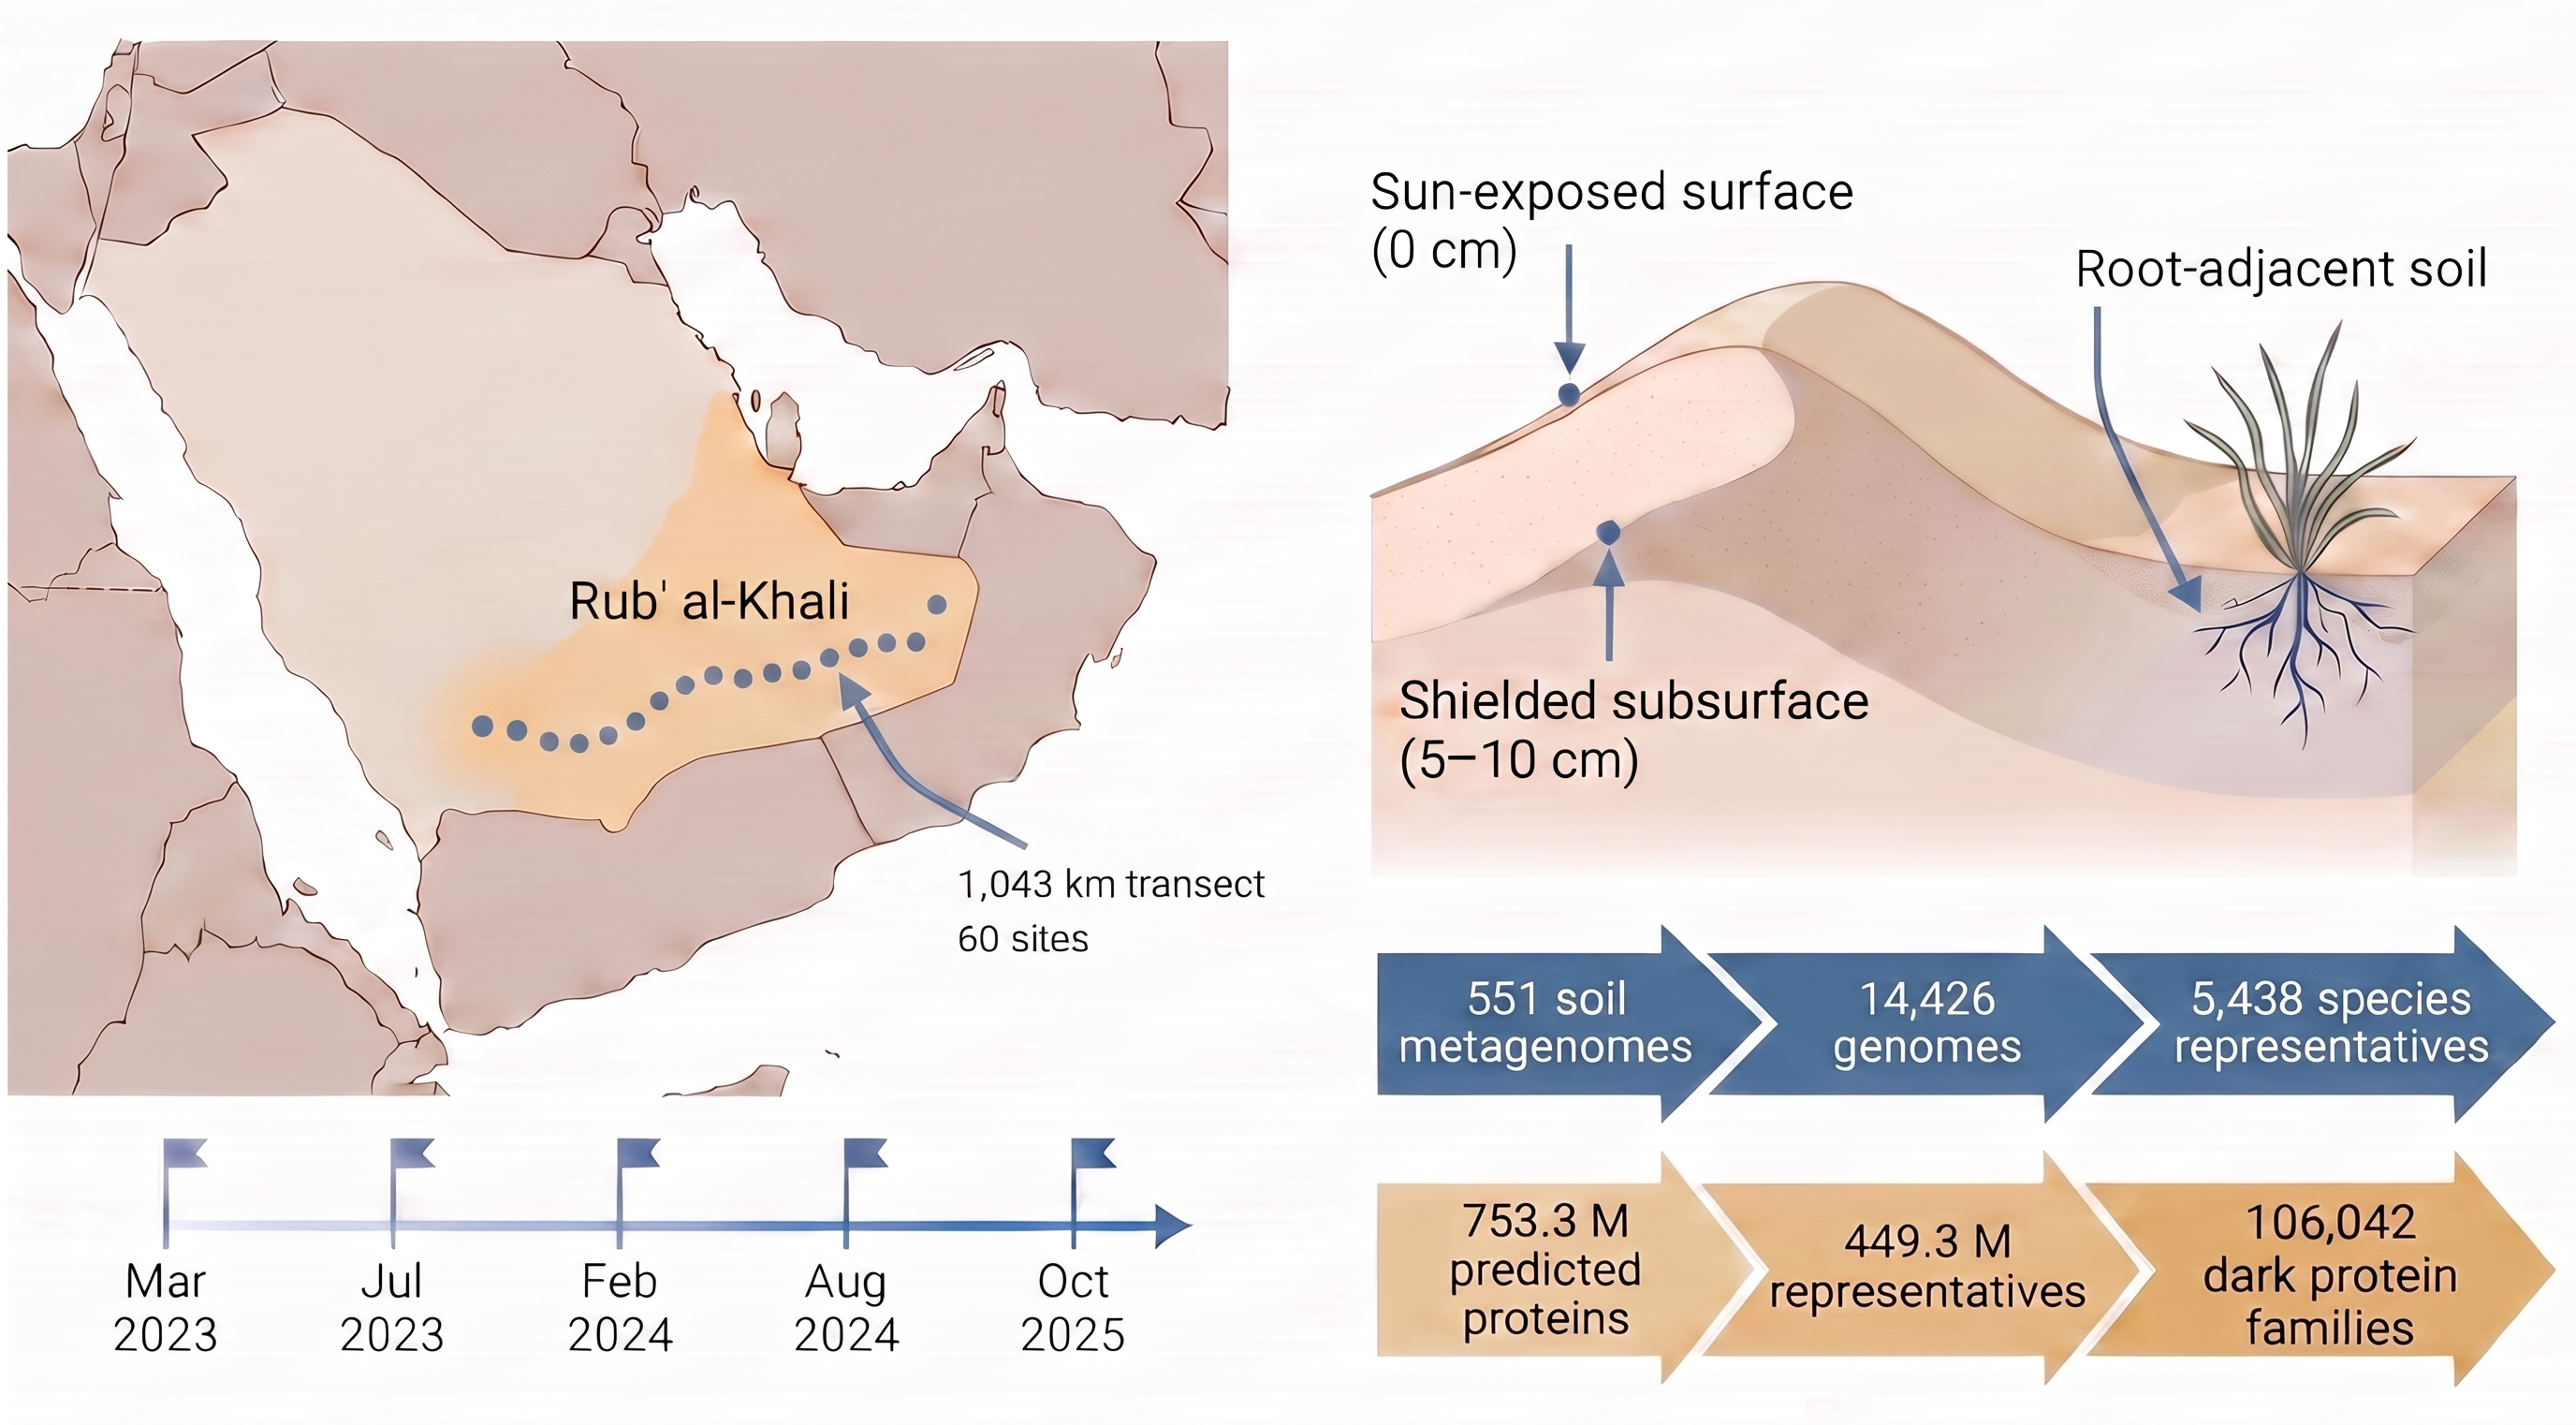
\includegraphics[width=\textwidth]{figures/fig_study_design.png}
\caption{\textbf{Study design and catalogue.} \textbf{a}, The 60 sites along the 1{,}043~km transect.
\textbf{b}, Five expeditions between March 2023 and October 2025. \textbf{c}, Three soil positions,
surface (0~cm), subsurface (5--10~cm) and root-adjacent (5--10~cm), and the 551 samples by position.
\textbf{d}, From 549 assemblies through two binnings and refinement to 14{,}426 bins and 5{,}438
species representatives. \textbf{e}, First empty rank of the 5{,}438 representatives under GTDB
release 232: none at domain, phylum or class; 11 at order, 142 at family, 1{,}343 at genus, 3{,}755
at species, 187 named to species.\todo{redraw in vector to these panels; the current file is the v1
draft illustration}}
\label{fig:design}
\end{figure}

\begin{figure}[p]\centering
\fbox{\parbox{0.9\textwidth}{\centering\vspace{6em}Figure 2: to be built from
\texttt{darkfam\_basis\_clean} and \texttt{cultured\_comparison\_clean}\vspace{6em}}}
\caption{\textbf{The reference-absent tenth of the protein clusters behaves as coding sequence.}
\textbf{a}, The census with its denominator at each step: 449{,}265{,}306 cluster representatives,
69{,}938{,}628 (15.6\%) with no UniRef50 hit, 43{,}423{,}322 with a member on a contig of a
medium- or high-quality bin, 4{,}292{,}446 (9.89\%) of those dark. \textbf{b}, Length and gene-call
completeness of dark against all representatives: length separates them (76\% against 30\% under
100 residues), completeness does not (86.7\% against 87.5\% partial). \textbf{c}, Expedition
persistence of the 106{,}042 dark families by read recruitment (79.4\% in all five) and by
independent assembly (28.9\%), within length strata. \textbf{d}, Median pairwise dN/dS per family
for 97{,}200 dark and 95{,}647 length- and size-matched UniRef50-matched control families (medians
0.425 and 0.388), with the frame-shifted null on a 10{,}000-family subset (median 1.087) and the same
subset in the annotated frame (0.427). \textbf{e},
Dark fraction of 23 soil species in cultured long-read genomes against their catalogue
representatives, paired by species.}
\label{fig:dark}
\end{figure}

\begin{figure}[p]\centering
\fbox{\parbox{0.9\textwidth}{\centering\vspace{6em}Figure 3: to be built from
\texttt{lineage\_darkness\_clean}\vspace{6em}}}
\caption{\textbf{Lineage sets the unknown fraction of a genome, and two archaeal classes carry a
fifth of it.} \textbf{a}, Variance in per-genome dark fraction explained by assembly quality alone,
quality plus phylum, and quality plus phylum plus genus, over the 5{,}438 representatives.
\textbf{b}, Median dark fraction by first unnamed rank. \textbf{c}, Residual dark fraction after the
quality model, by phylum (phyla with at least 20 representatives). \textbf{d}, Dark fraction of the
237 Thermoplasmatota representatives against their 1:1 matches among other archaea and among
bacteria, matched on completeness, contamination, corrected size, N50, abundance and prevalence.
\textbf{e}, Occurrence of the two classes across samples and soil positions.\todo{all panel values
enter after registration}}
\label{fig:lineage}
\end{figure}

\begin{figure}[p]\centering
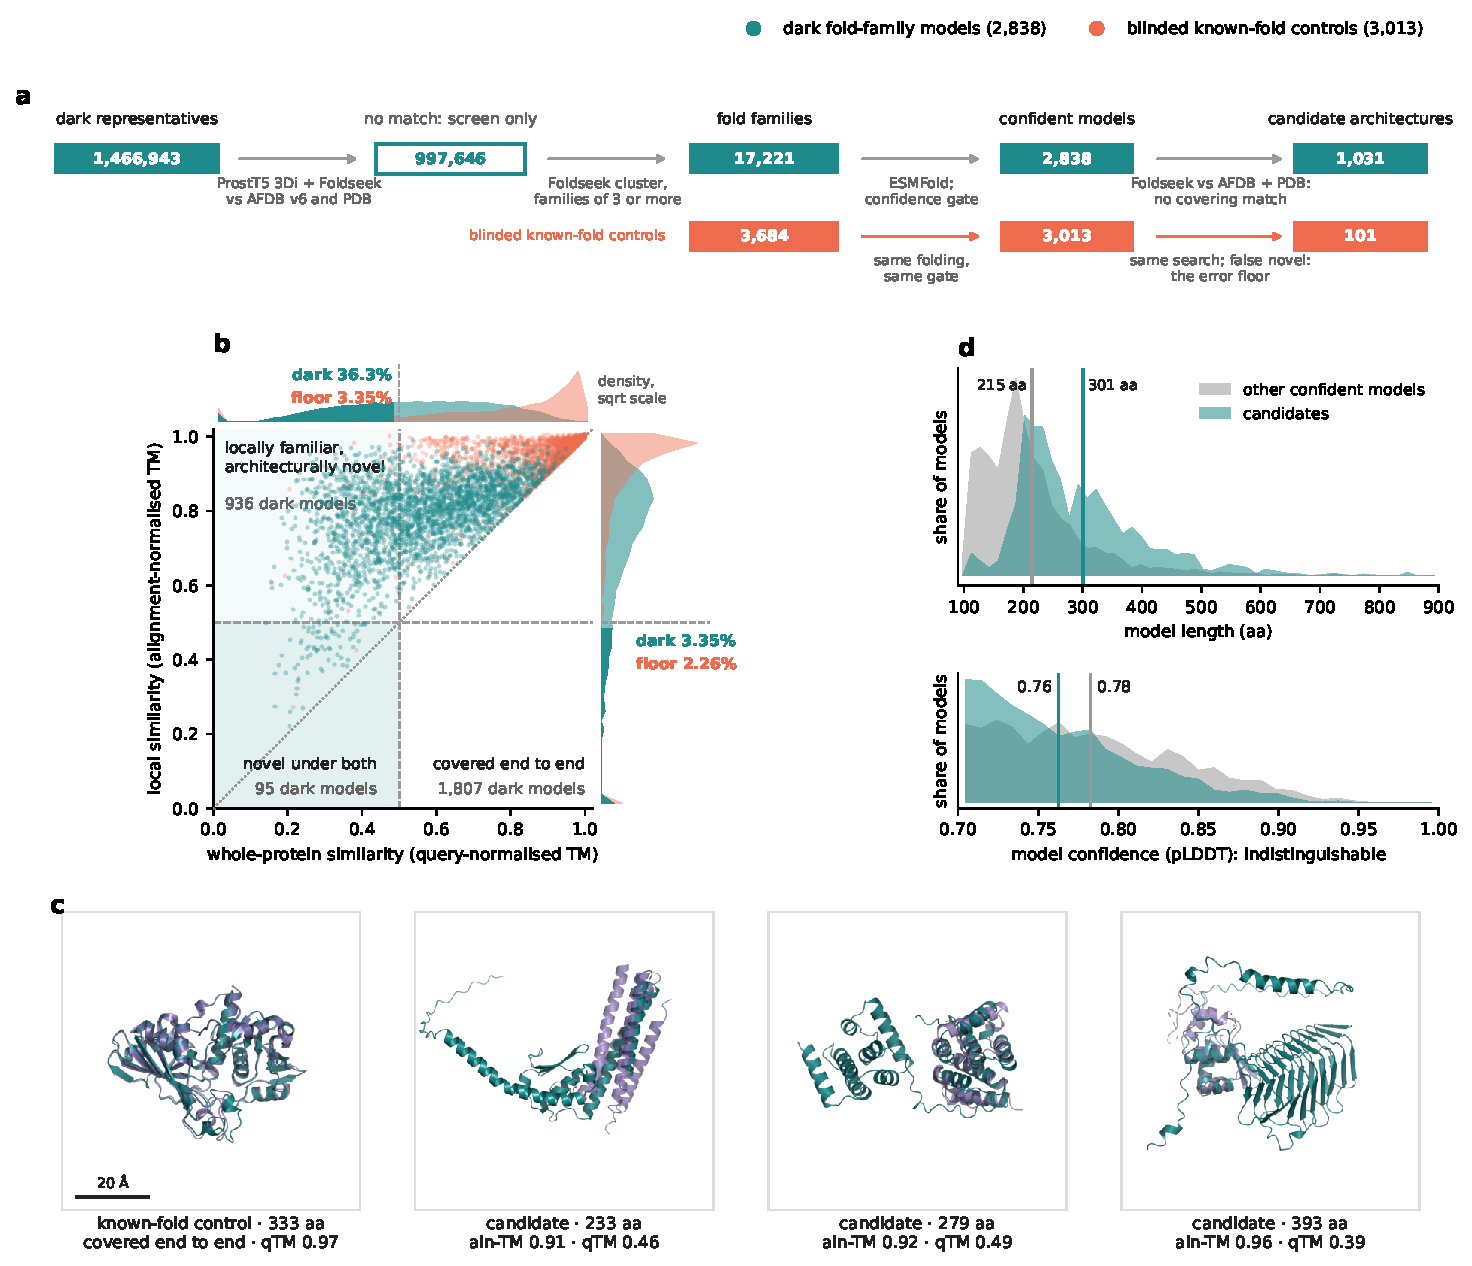
\includegraphics[width=\textwidth]{figures/fig_structural_calibration.pdf}
\caption{\textbf{Structural novelty is architectural, not local, against a blinded floor.}
\textbf{a}, From 1{,}466{,}943 genome-resolved dark representatives of at least 100 residues to
1{,}031 candidate architectures: 3Di triage against the AlphaFold Database v6 and the PDB (hollow box,
a triage, not a result), structural clustering, admission at three or more members, one ESMFold model
per family, the confidence gate, and the coordinate screen against the same references with 3{,}684
blinded known-fold controls (1{,}777 complete PDB chains, 1{,}907 deterministic crops) in the same run.
\textbf{b}, Best whole-protein similarity (query-normalised TM-score) against best local similarity
(alignment-normalised TM-score) for the 2{,}838 confident dark models and the 3{,}013 gate-passing
controls; dashed lines mark 0.5. Marginal densities give 36.3\% (95\% CI 34.6--38.1) of dark models
below threshold on the whole-protein axis against a 3.35\% control floor, and 3.35\% against 2.26\%
on the local axis. Standardised to the candidates' confidence and length, the whole-protein excess is
6.6 to 8.1 times the floor and the local excess is 1.38 with an interval crossing one. \textbf{c},
Superpositions of query models (teal) on the matched part of the nearest known structure (violet), at
one scale (bar, 20~\AA): the median covered control and three confident candidates in three length
bands. \textbf{d}, Model length and mean pLDDT for the 1{,}031 candidates and the 1{,}807 other
confident dark models. Candidates are reference- and metric-relative, not validated folds.}
\label{fig:structural}
\end{figure}

\begin{figure}[p]\centering
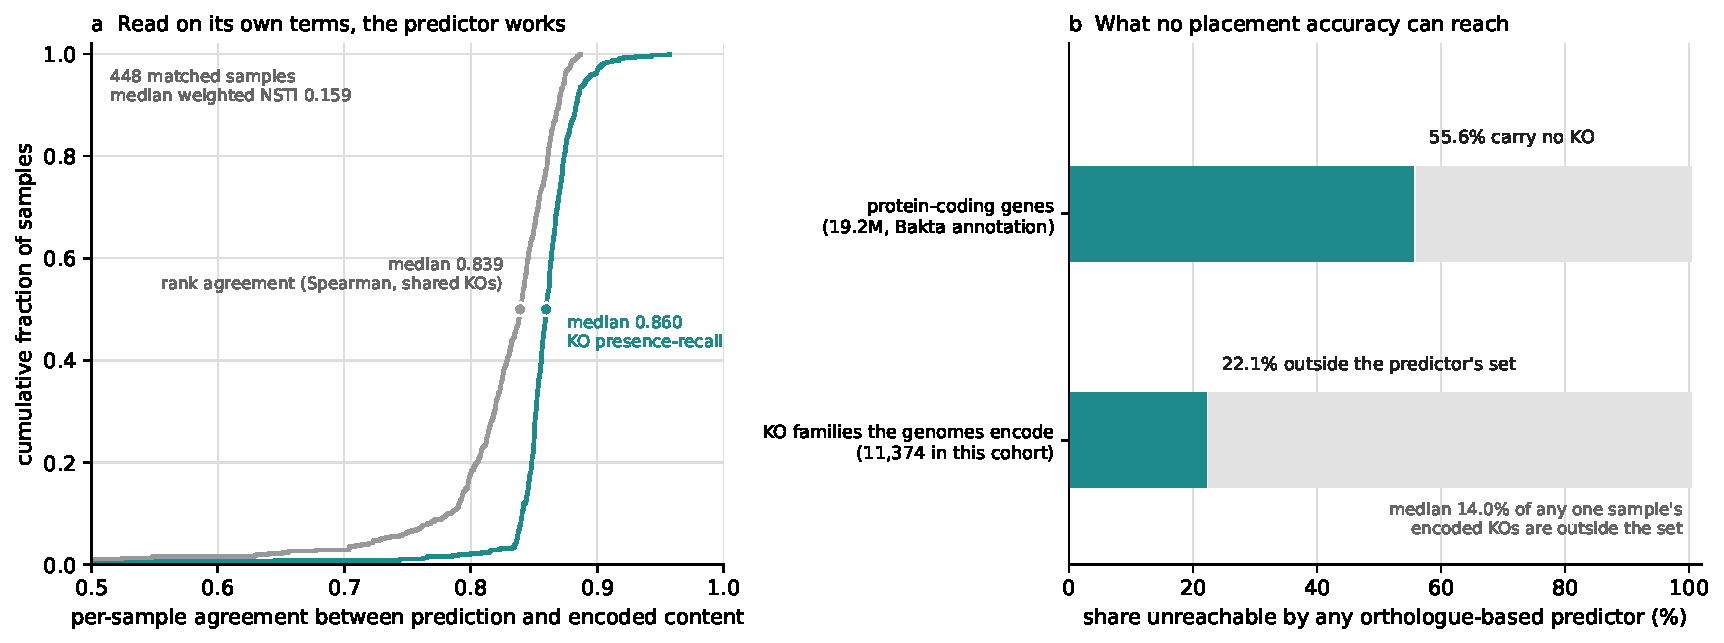
\includegraphics[width=0.9\textwidth]{figures/fig_refbias_ceiling.pdf}\\[1em]
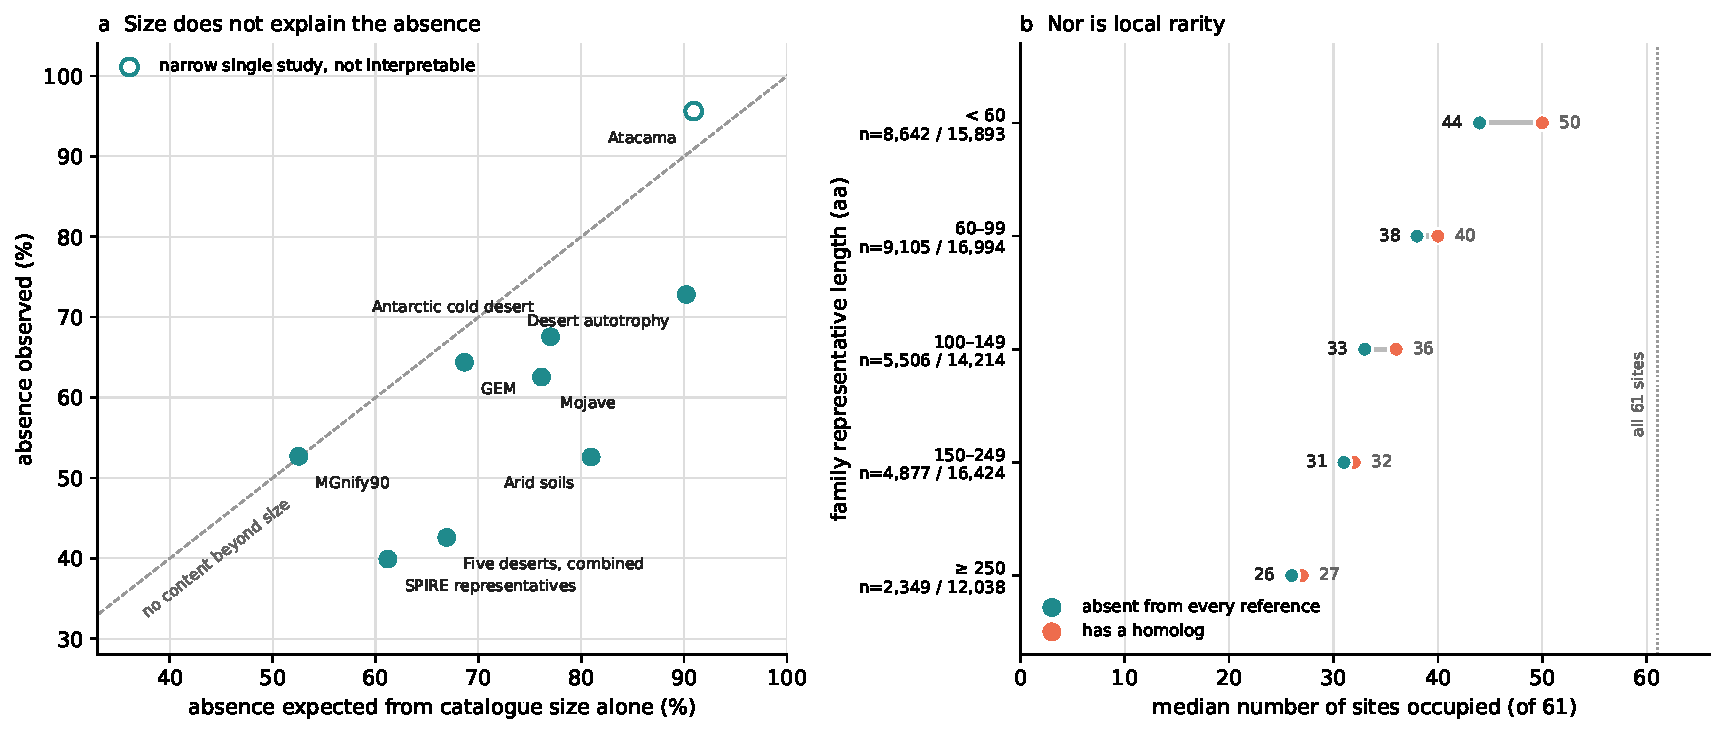
\includegraphics[width=0.95\textwidth]{figures/fig_specificity_controls.pdf}
\caption{\textbf{The gap is in the reference set.} \textbf{a}, Per-sample agreement between
marker-gene prediction and genome-encoded content over 448 samples: presence-recall (median 86.0\%)
and rank agreement on shared orthologues (median Spearman $\rho$ 0.839); the two ceilings, 55.6\% of
protein-coding genes with no orthologue and 22\% of encoded orthologues outside the predictor's set.
\textbf{b}, Observed absence of the 106{,}042 dark families and their matched controls from each
catalogue against the absence expected from catalogue size alone (E-value-corrected rarefaction of
MGnify90). The diagonal is the size-only expectation; a point below it holds more relevant sequence
than its size predicts. MGnify90 sits on the diagonal by construction. The Atacama study is drawn
open: its control gap of $-29.97$ points shows that a single 35-sample study samples protein space
too narrowly to beat a random draw even for conserved proteins. \textbf{c}, Median occupancy over
the 61 sampled locations of dark families absent from every catalogue (37) and of those with a hit
(38), within length strata. Absence is database-relative under the stated rule and is not geographic
absence.}
\label{fig:reference}
\end{figure}

\begin{figure}[p]\centering
\includegraphics[width=0.48\textwidth]{figures/fig_darkmatter_pcoa.pdf}\hfill
\includegraphics[width=0.48\textwidth]{figures/fig_darkmatter_permanova.pdf}\\[1em]
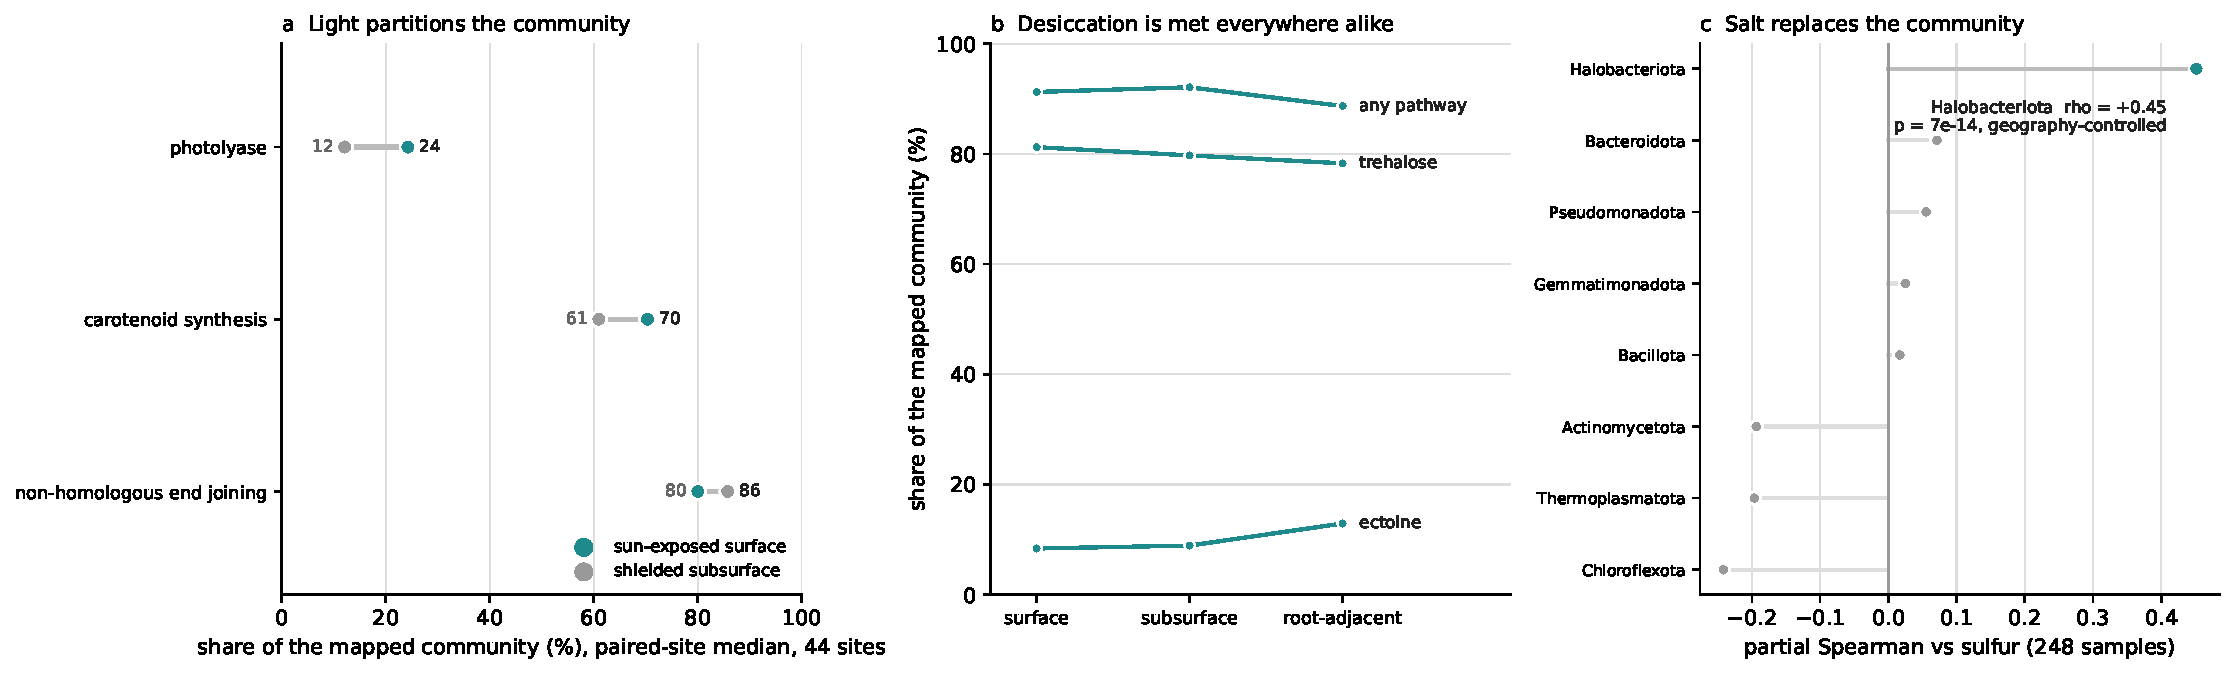
\includegraphics[width=\textwidth]{figures/fig_stress_modes.pdf}
\caption{\textbf{Geochemistry structures known and unknown gene content beyond distance.}
\textbf{a}, Principal coordinates of 547 samples on Bray--Curtis dissimilarity of Hellinger-transformed
dark-family abundance, coloured by aridity index and by soil position. \textbf{b}, PERMANOVA variance
explained per block, marginal and conditioned on space; every block $p = 0.001$ except the single-axis
vanadium control ($p = 0.78$).\todo{rebuild panel b on the corrected eleven-axis geochemistry block
(0.132 / 0.089) and add the three-block partition; the current file shows the superseded block}
\textbf{c}, Site-paired share of the mapped community carrying photolyase, carotenoid synthesis and
non-homologous end joining, surface against subsurface (44 sites). \textbf{d}, Compatible-solute
capacity is uniform across positions. \textbf{e}, Partial Spearman correlation of each phylum's share
with sulfur, geography-controlled (248 samples); Halobacteriota alone tracks the salt axis. Genomic
capacities and DNA-based abundances, not measured activity.}
\label{fig:environment}
\end{figure}

\bibliographystyle{unsrtnat}
\bibliography{references}

\end{document}
